\documentclass[12pt, twoside]{article}
\usepackage[utf8]{inputenc}
\usepackage[english,russian]{babel}

\usepackage{amsthm}
\usepackage{a4wide}
\usepackage{graphicx}
\usepackage{caption}
\usepackage{subcaption}
\usepackage{amssymb}
\usepackage{amsmath}
\usepackage{mathrsfs}
\usepackage{euscript}
\usepackage{graphicx}
\usepackage{caption}
\usepackage{color}
\usepackage{bm}
\usepackage{tabularx}
\usepackage{adjustbox}


\usepackage[toc,page]{appendix}

\usepackage{comment}
\usepackage{rotating}

\DeclareMathOperator*{\argmax}{arg\,max}
\DeclareMathOperator*{\argmin}{arg\,min}

\newtheorem{theorem}{Теорема}
\newtheorem{lemma}[theorem]{Лемма}
\newtheorem{definition}{Определение}[section]

\numberwithin{equation}{section}

\newcommand*{\No}{No.}
\begin{document}

\title{\bf Анализ свойств вероятностных моделей в задачах обучения с экспертом}
\date{}
\author{}
\maketitle

\begin{center}
\bf
А.\,И. Базарова\footnote{Московский физико-технический институт, bazarova.ai@phystech.edu}, А.\,В.~Грабовой\footnote{Московский физико-технический институт, grabovoy.av@phystech.edu}, В.\,В.~Стрижов\footnote{Московский физико-технический институт, strijov@ccas.ru}

\end{center}

{\centering\begin{quote}
\textbf{Аннотация:} Данная работа посвящена построению интерпретируемых моделей в машинном обучении.
Решается задача аппроксимации заданного набора фигур на контурном изображении.
Вводятся предположения о том, что фигуры являются кривыми второго порядка.
При аппроксимации фигур используется информация о типе, расположению и виде кривых, а также о множестве их возможных преобразований.
Такая информация называется \textit{экспертной}, а метод машинного обучения, основанный на экспертной информации, называется \textit{обучением с экспертом}.
Предполагается, что набор фигур аппроксимируется набором \textit{локальных моделей}.
Каждая локальная модель на основе экспертной информации аппроксимирует одну фигуру на контурном изображении.
Для построение моделей предлагается отобразить кривые второго порядка в признаковое пространство, в котором каждая локальная модель является линейной моделью.
Таким образом, кривые высших порядков расспознаются при помощи композиции линейных моделей.
В качестве прикладной задачи рассматривается задача аппроксимации радужки глаза на контурном изображении.
    
\smallskip
\textbf{Ключевые слова}: смесь экспертов, обучение с экспертом, линейные модели, интерпретируемые модели
\smallskip
\textbf{DOI}: 00.00000/00000000000000
\end{quote}
}

\section{Введение}
Построения интерпретируемых моделей в машинном обучении~\cite{Ribeiro2016} является одной из ключевых проблем.
Современные решения задачи классификации изображений на основе сетей глубокого обучения ResNet, VGG, Intercept~\cite{Kaiming2015} являются плохо интерпретируемыми моделями.
В работах~\cite{Han2020, Xingjun2019, Akhtar2018} показано, что сети глубоко обучения чувствительны даже к малому шуму в данных, что связано с их неинтерпретируемостью.

В данной работе предлагается метод \textit{обучения с экспертом}.
Данные метод предполагает использование предметных знаний экспертов для повышения качества аппроксимации, а также для получения интерпретируемых моделей машинного обучения.
Предметные знание экспертов о выборке назовем~\textit{экспертной информацией}.
Предполагается, что использования экспертной информации позволяет аппроксимировать выборку простыми интерпретируемыми моделями, например линейными моделями. Методы машинного обучения, которые учитывают экспертные знания при построении моделей, назовем~\textit{обучением с экспертом}.

В работе решается задача аппроксимации кривых второго порядка на контурном изображении. Кривые второго порядка выбраны для анализа, так как они легко описываются линейными моделями. При этом данные фигуры требуется восстановить в таких прикладных задачах, как задача распознавания радужки глаза~\cite{Matveev2010, Matveev2014, Bowyer2010}, задача описания трека частицы в адронном коллайдере~\cite{Dalila}. Экспертная информация о кривой второго порядка позволяет отобразить точки на плоскости в новое признаковое описание, в котором каждая кривая аппроксимируется одной линейной моделью. Модель, которая аппроксимирует одну кривую называется \textit{локальной моделью}. Для аппроксимации всего контурного изображения требуется аппроксимировать несколько кривых второго порядка при помощи нескольких локальных моделей. В данной работе вводятся следующие ограничения на изображения:
\begin{enumerate}
	\item[1)] изображение состоит только из кривых второго порядка;
	\item[2)] изображение аппроксимируется малым числом кривых второго порядка;
	\item[3)] число и тип кривых на изображении известно.
\end{enumerate}

\begin{figure}
     \centering
     \begin{subfigure}[b]{0.3\textwidth}
         \centering
         \includegraphics[width=\textwidth]{figures/explanation_exp1}
         \caption{}
         \label{intro:fig2:exp1}
     \end{subfigure}
     \begin{subfigure}[b]{0.3\textwidth}
         \centering
         \includegraphics[width=\textwidth]{figures/explanation}
         \caption{}
         \label{intro:fig2:image}
     \end{subfigure}
     \begin{subfigure}[b]{0.3\textwidth}
         \centering
         \includegraphics[width=\textwidth]{figures/explanation_exp2}
         \caption{}
         \label{intro:fig2:exp2}
     \end{subfigure}

     \caption{Пример: a) представления данных первым экспертом; b) исходные данные; c) представления данных вторым экспертом.}
    \label{intro:fig1}
\end{figure}

При аппроксимации нескольких кривых на одном контурном изображении строится мультимодель. Примером мультимоделей является случайный лес~\cite{Ishwaran2012}, бустинг деревьев~\cite{Tianqi2016}, смесь экспертов~\cite{Yuksel2012}. В данной работе в качестве мультимодели рассматривается смесь экспертов. Смесь экспертов~---~это мультимодель, которая линейно взвешивает локальные модели, которые аппроксимируют часть выборки. Значения весовых коэффициентов зависят от того объекта, для которого производится предсказание. Для решения задачи смеси экспертов используется вариационный ЕМ-алгоритм~\cite{Dempster1977, bishop2006, Peng1996}. Смесь экспертов имеет множество применений в ряде прикладных задач. В работе~\cite{Estabrooks2001} решается задача классификации текстов. В работах~\cite{Cheung1995, Weigend2000, Cao2003, Mossavat2010, Sminchisescu2007, Tuerk2001, Yumlu2003} смесь экспертов используется для предсказания временных рядов в задачах распознавания речи, дневной активности человека и предсказания стоимости ценных бумаг. В работе~\cite{Ebrahimpour2009} смесь экспертов рассматривался для решения задачи распознавания рукописных цифр на изображениях.

В качестве примера рассматривается задача аппроксимации изображения радужки глаза. На рис.~\ref{intro:fig1:real} показан пример изображения, которое требуется аппроксимировать. В данной работе рассматривается обработанное изображение, которое приведено в контурный вид, пример такого изображение показан на рис.~\ref{intro:fig1:outer}. На рис.~\ref{intro:fig1:outer} показаны две локальные модели окружностей, которые аппроксимируют радужку глаза. Окружности являются простым примером кривой второго порядка.

\begin{figure}
     \centering
     \begin{subfigure}[b]{0.3\textwidth}
         \centering
         \includegraphics[width=\textwidth]{figures/real_image}
         \caption{}
         \label{intro:fig1:real}
     \end{subfigure}
     \begin{subfigure}[b]{0.3\textwidth}
         \centering
         \includegraphics[width=\textwidth]{figures/outline_image}
         \caption{}
         \label{intro:fig1:outer}
     \end{subfigure}
     \caption{Пример изображении радужки глаза и его контурного представления: a) изображение радужки глаза; b) контурное изображение радужки и аппроксимирующие данное изображение окружности.}
    \label{intro:fig1}
\end{figure}

Для задачи аппроксимации радужки глаза используется следующая экспертная информация: радужка глаза аппроксимируется двумя концентрическими окружностями. Экспертная информация используется при построении признакового описания точек плоскости, а также при построении функции оптимизации. Часть функции ошибки для оптимизации, которая использует экспертную информации называется регуляризатором. Таким образом информация о том, что на изображении окружности задается признаковым описанием, а информация о том, что окружности концентрические задается при помощи специального регуляризатора.

В вычислительном эксперименте проводится анализ качества аппроксимации контурного изображения в зависимости от заданной экспертной информации и от уровня шума в синтетически сгенерированных данных. Проводится анализ качества аппроксимации радужки глаза в зависимости от количества экспертной информации, которая использовалась при построении модели. Заметим, что каждое аппроксимируемое изображение это отдельный набор точек, которые требуется аппроксимировать.


\section{Постановка задачи нахождения параметров кривых второго порядка на изображении}
Задано бинарное изображение:
$$ \mathbf{M} \in \{0, 1 \}^{m_1\times m_2},$$
где 1 отвечает черной точке изображения, а 0~---~белой точке фона.
По изображению $\mathbf{M}$ строится выборка $\mathbf{C}$, элементами которой являются координаты $(x_i, y_i)$ черных точек: $$\mathbf{C} \in \mathbb{R}^{N \times 2}.$$
Эксперт предполагает, что изображение состоит из кривой второго порядка~$\Omega$.
Пусть для набора точек $\mathbf{C} \in \mathbb{R}^{N \times 2}$, образующих кривую $\Omega,$ задано экспертная информация о фигуре $E(\Omega)$.
Множество $E(\Omega)$ состоит из ожидаемого экспертом вида фигуры $\Omega$ и множества ее допустимых преобразований. На основе экспертного описания введем отображения в новую задачу для аппроксимации:
\begin{equation}\label{eq1}
	K_{x}\bigl(E(\Omega)\bigr): \mathbb{R}^{2} \rightarrow \mathbb{R}^{n}, \quad K_{y}\bigl(E(\Omega)\bigr): \mathbb{R}^{2} \rightarrow \mathbb{R},
\end{equation} 
где~$K_{x}$ отображение объекты в признаковое описание объектов,~$n$~--- число признаков, а~$K_{y}$ отображение в целевую переменную для объекта. Применив отображения~$K_{x},K_{y}$ для выборки~$\mathbf{C}$ поэлементно получаем:
\begin{equation}
\label{eq2}
	K_{x}\bigl(E(\Omega\bigr), \mathbf{c}) = \mathbf{x}, \quad  K_{y}\bigl(E(\Omega), \mathbf{c}\bigr) = y,
\end{equation}
где~$\mathbf{c} = (x_i, y_i)$~---~точка из выборки $\mathbf{C}$.

Применяя отображения \eqref{eq2} к исходному набору точек $\mathbf{C}$, получим выборку 
\begin{equation}
\label{eq4}
    \mathfrak{D} = \{(\mathbf{x}, y) \; | \; \forall \mathbf{c} \in \mathbf{C} \; \mathbf{x} = K_x(\mathbf{c}), \; y = K_y(\mathbf{c}) \}.
\end{equation}

Получаем, что исходная задача аппроксимации кривой~$\Omega$ сводится к аппроксимации выборки~$\mathfrak{D}$. В данной работе предполагается, что выборка~$\mathfrak{D}$ аппроксимируется линейной моделью:
\begin{equation}
	g(\mathbf{x}, \mathbf{w}) = \mathbf{x}^\mathsf{T} \mathbf{w},
\end{equation} 
где~$\mathbf{w}$ вектор, параметр, который требуется найти.

Для поиска оптимального вектора параметров~$\hat{\mathbf{w}}$ требуется решить следующую оптимизационную задачу:
\begin{equation}
	\hat{\mathbf{w}} = \arg\min_{\mathbf{w}\in\mathbb{R}^n} \sum_{\left(\mathbf{x}, y\right) \in \mathfrak{D}}\|g(\mathbf{x}, \mathbf{w}) - y \|_2^2.
\end{equation} 

Таким образом, задача аппроксимации исходной кривой~$\Omega$ сводится к решению задачи линейной регрессии, т.~е. нахождения компонент вектора $\hat{\mathbf{w}}$, связывающего полученные $\mathbf{x}$ и $y$.

В случае, когда на изображении $K$ кривых второго порядка  $\Omega_1, \dots, \Omega_K$, для каждой из которых имеется экспертная информация $E_k = E(\Omega_k), \, k \in \{1, \dots, K\}$, ставится задача построения мультимодели, называемой смесью $K$ экспертов. 

\begin{definition}
Назовем мультимодель $f$ смесью K экспертов
\begin{equation}
	f = \sum\limits_{k = 1}^{K}\pi_k(\mathbf{x}, \mathbf{V})g_k(\mathbf{w}_k),  \quad \pi_k(\mathbf{x}, \mathbf{V}): \mathbb{R}^{n\times |\mathbf{V}|} \rightarrow [0, \, 1], \quad \sum\limits_{k = 1}^{K}\pi_k(\mathbf{x}, \mathbf{V}) = 1, 
\end{equation}
где $g_k$~---~локальная модель, называемая экспертом, $\mathbf{x}$~---~признаковое описание объекта, $\pi_k$~---~шлюзовая функция, вектор $\mathbf{w}_k$~---~параметры локальной модели, вектор $\mathbf{V}$~---~параметры шлюзовой функции. В данной работе $g_k$~---~линейная модель.
\end{definition}

Для каждой кривой второго порядка заданы отображения (\ref{eq1}). Для удобства введем следующее обозначение: $K_x^k\bigr(\mathbf{c}\bigr) = K_x\bigr(\Omega_k, \mathbf{c}\bigr)$ и $K_y^k\bigr(\mathbf{c}\bigr) = K_y\bigr(\Omega_k, \mathbf{c}\bigr)$. Тогда, используя локальные линейные модели, построим универсальную мультимодель, описывающую кривые $\Omega_1, \dots, \Omega_K$ на изображении $\mathbf{M}$:
\begin{equation}
\label{5}
	f = \sum\limits_{\mathbf{c} \in \mathbf{C}} \sum_{k = 1}^{K} \pi_k(\mathbf{c}, \mathbf{V})g_k(K^k_{x}\bigl(\mathbf{c}), \mathbf{w}_k), 
\end{equation}
где $\pi_k$~---~шлюзовая функция. В данной работе рассмотривается простой случай, когда~$\mathbf{x}=K^1_{x}\bigl(\mathbf{c})=\cdots=K^K_{x}\bigl(\mathbf{c}),$ тогда выражение~\eqref{5} переписывается в следующем простом виде:
\begin{equation}
\label{5_1}
	f = \sum\limits_{\mathbf{c} \in \mathbf{C}} \sum_{k = 1}^{K} \pi_k(\mathbf{x}, \mathbf{V})g_k(\mathbf{x}, \mathbf{w}_k), 
\end{equation}
где шлюзовая функция $\pi_k$ имеет следующий вид:
\begin{equation}
\label{6}
	\pi_k(\mathbf{x}, \mathbf{V}): \mathbb{R}^{n\times |\mathbf{V}|} \rightarrow [0, \, 1], \; \; \; \; \sum\limits_{k = 1}^{K}\pi_k(\mathbf{x}, \mathbf{V}) = 1,
\end{equation}
где $\mathbf{V}$~---~параметры шлюзовой функции, а $g_k$~---~локальная модель.
    
В данной работе
\begin{equation}
    \boldsymbol{\pi}(\mathbf{x}, \mathbf{V}) = \text{softmax}\bigl(\mathbf{V}_1^{\mathsf{T}}\boldsymbol{\sigma}(\mathbf{V}_2^{\mathsf{T}}\mathbf{x}) \bigr),
\end{equation}
где $\mathbf{V} = \{ \mathbf{V}_1, \, \mathbf{V}_2\}$~---~параметры шлюзовой функции, $\mathbf{V}_1 \in \mathbb{R}^{p \times k}, \, \mathbf{V}_2 \in \mathbb{R}^{n \times p}$. 

Для нахождения оптимальных параметров мультимодели необходимо решить следующую задачу оптимизации:
\begin{equation}\label{9}
\mathcal{L} = \sum\limits_{(\mathbf{x}, y) \in \mathfrak{D}} \sum\limits_{k = 1}^{K} \pi_k(\mathbf{x}, \mathbf{V})(y - \mathbf{w}_k^{\mathsf{T}}\mathbf{x})^2 + R\bigl(\mathbf{V}, \mathbf{W}, E(\Omega)\bigr) \rightarrow \min_{\mathbf{V}, \mathbf{W}},
\end{equation}
где $\mathbf{W} = [\mathbf{w}_1, \dots, \mathbf{w}_k]$~--- параметры локальных моделей, $R\bigl(\mathbf{V}, \mathbf{W}, E(\Omega)\bigr)$~---~регуляризация параметров, основанная на экспертной информации.

\section{Построение признакового описания фигур}
\paragraph{Единое пространство для кривых второго порядка.} Произвольная кривая второго порядка, главная ось которой не параллельна оси ординат, задается следующим выражением:
\[
\label{st:coef}
x^2 = B'xy+C'y^2+D'x+E'y+F',
\]
где на коэффициенты $B',C'$ накладываются ограничения, которые зависят от вида кривой. Выражение~\eqref{eq2} принимает следующий вид:
\[
\label{st:K_map}
K_x\bigr(\mathbf{c}_i\bigr)=\left[x_iy_i, y_i^2, x_i, y_i, 1\right], \quad K_y\bigr(\mathbf{c}_i\bigr)=x_i^2,
\]
откуда получаем задачу линейной регрессии для восстановления параметров~$B', C', D', E', F'$ по составленной выборке.

\paragraph{Окружность.} Частным случаем кривой второго порядка, рассмотрим окружность.
Пусть $(x_0, y_0)$~---~центр окружности, которую необходимо найти на бинарном изображении $\mathbf{M}$, а $r$~--- ее радиус.
Элементы выборки $(x_i, y_i) \in \mathbf{C}$ являются геометрическим местом точек, которое аппроксимируется уравнением окружности:
\begin{equation}
(x_i - x_0)^2 + (y_i - y_0)^2 = r^2.
\end{equation}
Раскрыв скобки, получим:
\begin{equation}(2x_0)\cdot x_i + (2y_0)\cdot y_i + (r^2 - x_0^2 - y_0^2)\cdot 1 = x_i^2 + y_i^2 . 
\end{equation}
Тогда отображения (\ref{eq2}) примут вид:
\begin{equation}
\label{10}
K_{x}(\mathbf{c}_i) = [x_i, \, y_i, \, 1] = \mathbf{x}, \,  K_{y}(\mathbf{c}_i) = x_i^2+y_i^2 = y.
\end{equation} 
Поставим задачу линейной регрессии \eqref{eq4}.
Компоненты вектора $\mathbf{w} = [w_0, \, w_1, \, w_2]^\mathsf{T}$, связывающего $\mathbf{x}$ и $y$, восстанавливают параметры окружности: \begin{equation} x_0 = \frac{w_0}{2}, \; y_0 = \frac{w_1}{2}, \; r = \sqrt{w_3 + x_0^2 + y_0 ^2}.\end{equation}

\section{Композиция фигур}
Для построения композиции фигур воспользуемся выражением~\eqref{9}, которое принимает следующий вид:
\begin{equation} 
\label{statment:optim:task}
\begin{aligned}
\mathcal{L} = \sum\limits_{\mathbf{c} \in \mathbf{C}} \sum\limits_{k = 1}^{K} \pi_k(\mathbf{c}, \mathbf{V})\left(K^{k}_y\bigr(\mathbf{c}\bigr) - \mathbf{w}_k^{\mathsf{T}}K^{k}_x\bigr(\mathbf{c}\bigr)\right)^2 + R\bigl(\mathbf{V}, \mathbf{W}, E(\Omega)\bigr) \rightarrow \min_{\mathbf{V}, \mathbf{W}},
\end{aligned}
\end{equation} 
где~$K^{k}_x, K^{k}_y$ экспертное представление~$k$-го эксперта. Предполагая, что все кривые на изображении описываются одним признаковым описанием $\mathbf{x} = K^{1}_x\bigr(\mathbf{c}\bigr)=\cdots=K^{K}_x\bigr(\mathbf{c}\bigr), x= K^{1}_y\bigr(\mathbf{c}\bigr)=\cdots=K^{K}_y\bigr(\mathbf{c}\bigr),$ получаем следующую оптимизационную задачу:
\begin{equation} 
\label{statment:optim:task:simp}
\begin{aligned}
\mathcal{L} = \sum\limits_{\left(\mathbf{x}, y\right) \in \mathfrak{D}} \sum\limits_{k = 1}^{K} \pi_k(\mathbf{x}, \mathbf{V})\left(y - \mathbf{w}_k^{\mathsf{T}}\mathbf{x}\right)^2 + R\bigl(\mathbf{V}, \mathbf{W}, E(\Omega)\bigr) \rightarrow \min_{\mathbf{V}, \mathbf{W}},
\end{aligned}
\end{equation} 

В качестве регуляризатора~$R$ рассматриваются дополнительные ограничения на вектора параметров моделей. Для решения оптимизационной задачи~\eqref{statment:optim:task:simp} предлагается использовать EM--алгоритм.

\section{Вычислительный эксперимент}
Проведен вычислительный эксперимент для анализа качества моделей кривых второго порядка на изображении. Эксперимент разделе на несколько частей. В первой части проводится эксперимент с несколькими окружностями на изображении. В второй части проводится анализ сходимости метода в зависимости от уровня шума в данных и от заданой экспертной информации. В третий части проводится эксперимент по аппроксимации радужки глаза.

\subsection{Эксперимент с окружностями}
\begin{figure}[h!]
\begin{minipage}{.32\textwidth}
      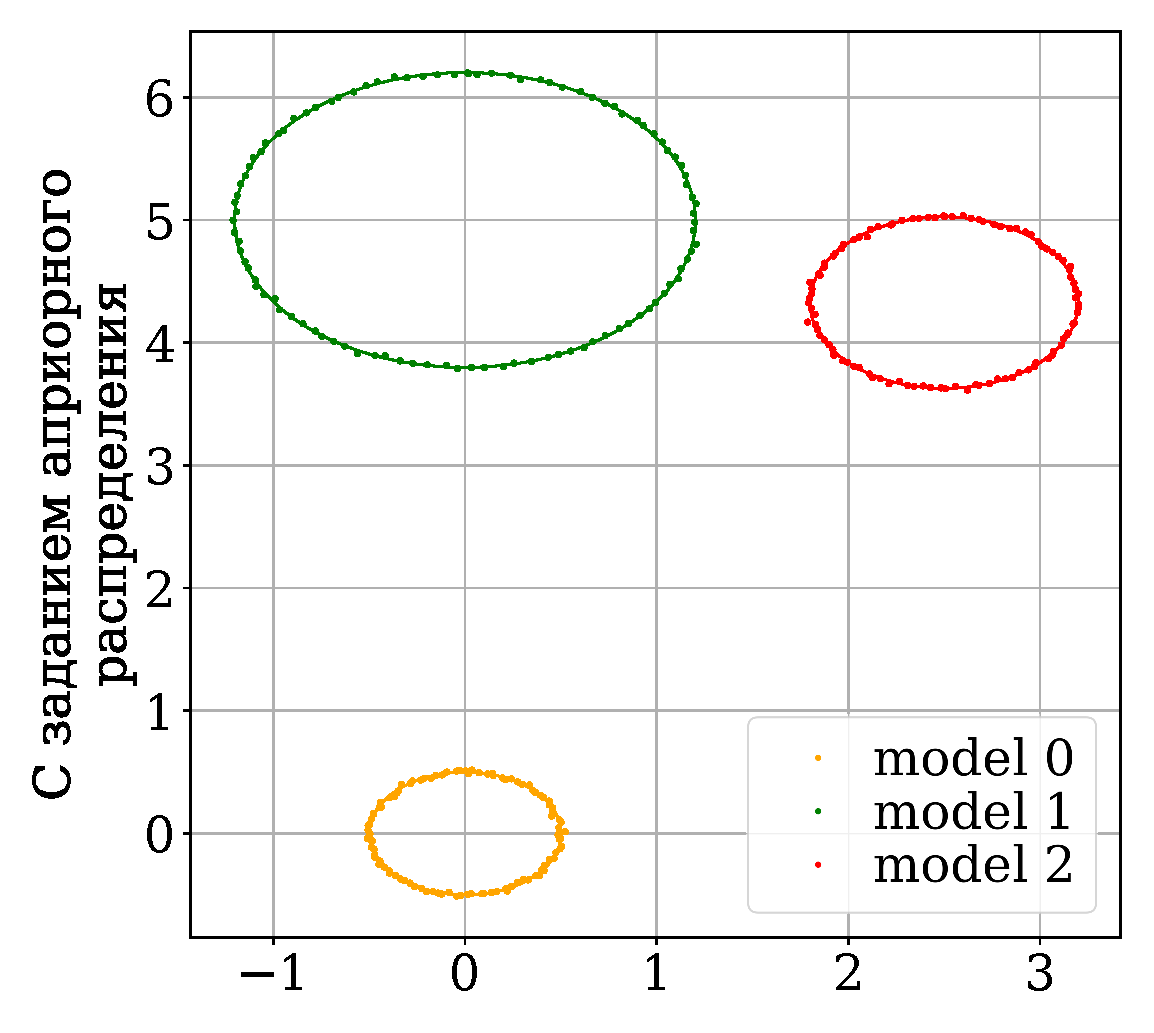
\includegraphics[width =  \textwidth]{figures/910.eps}
\end{minipage}
\begin{minipage}{.32\textwidth}
\hspace{0.3mm}
      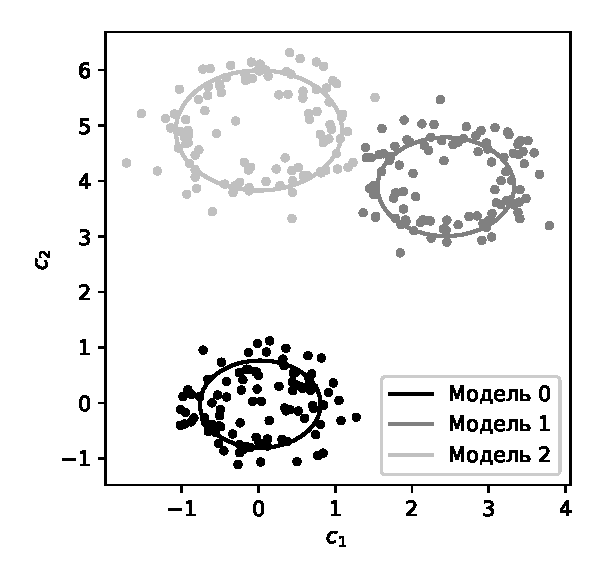
\includegraphics[width =  0.89\textwidth]{figures/901.eps}
\end{minipage}
\begin{minipage}{.32\textwidth}
\vspace{-3mm}
\hspace{-8.5mm}
      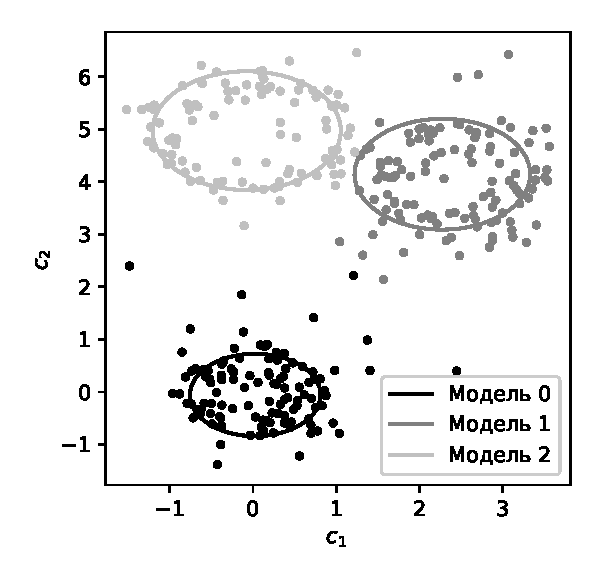
\includegraphics[width =  1.07\textwidth]{figures/902.eps}
\end{minipage}
\begin{minipage}{.32\textwidth}
      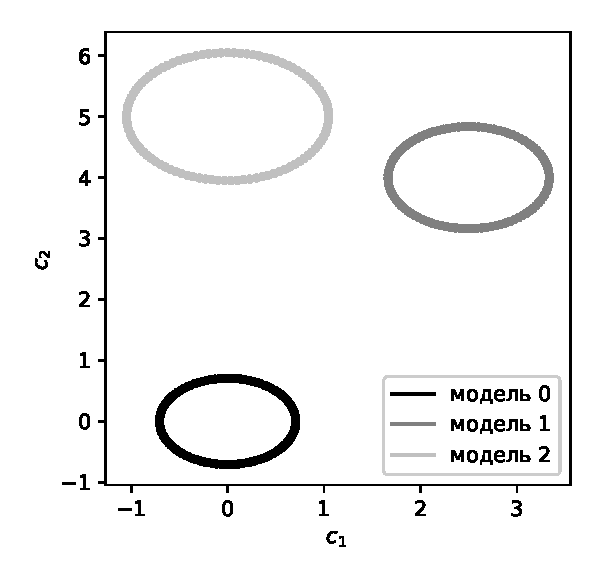
\includegraphics[width =  \textwidth]{figures/900.eps}
\end{minipage}
\begin{minipage}{.32\textwidth}
\hspace{2mm}
      \includegraphics[width =  0.9\textwidth]{figures/911.eps}
\end{minipage}
\begin{minipage}{.32\textwidth}
\hspace{-2.3mm}
      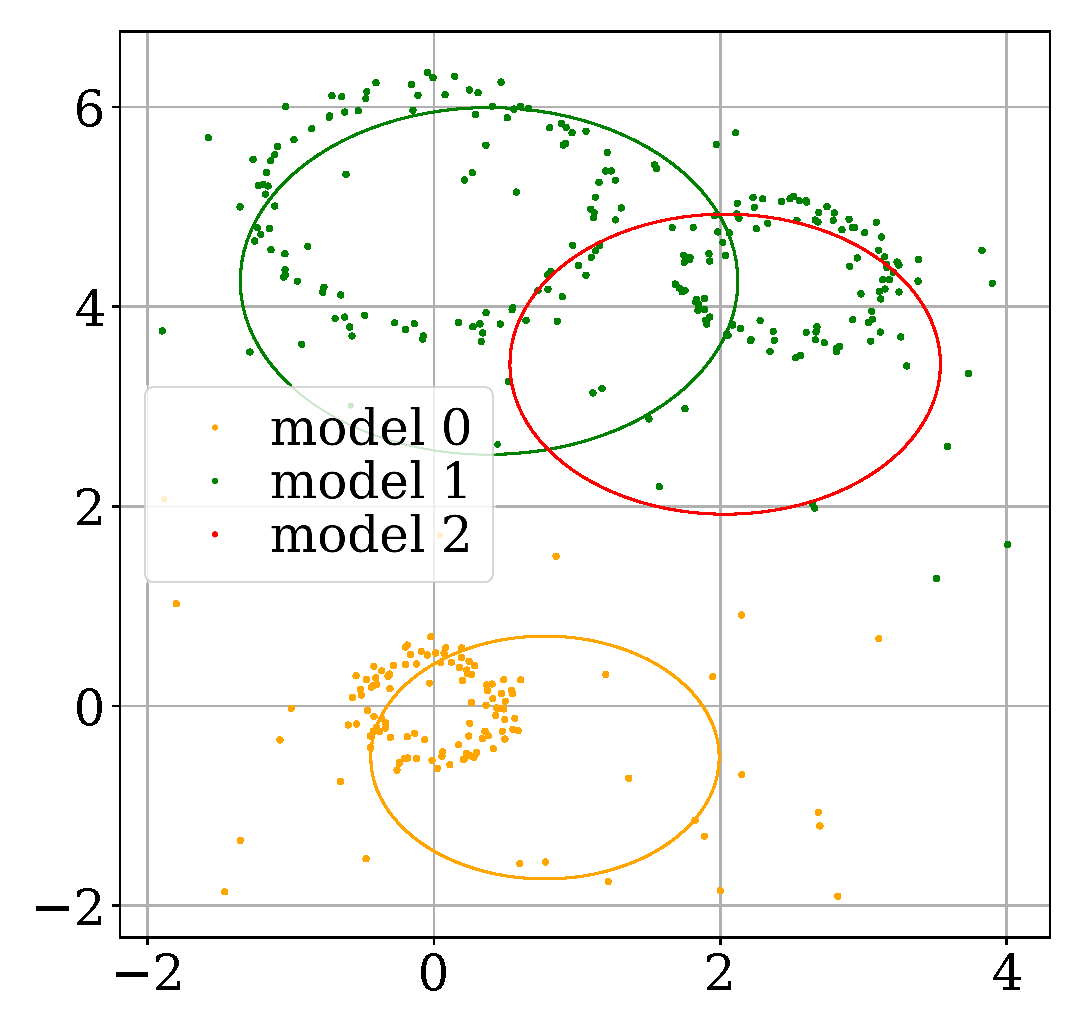
\includegraphics[width =  0.935\textwidth]{figures/912.eps}
\end{minipage}
\caption{Мультимодель в зависимости от разных априорных предположений и уровня шума. Сверху вниз: построение с заданием априорного распределения; без задания априорного распределения. Слева на право: окружности без шума; шум в радиусе окружности; шум в радиусе окружности а также произвольные точки по всему изображению.}
\label{ce:fig3}
\end{figure}

\begin{figure}[h]
\begin{minipage}{.32\textwidth}
\hspace{-3mm}
      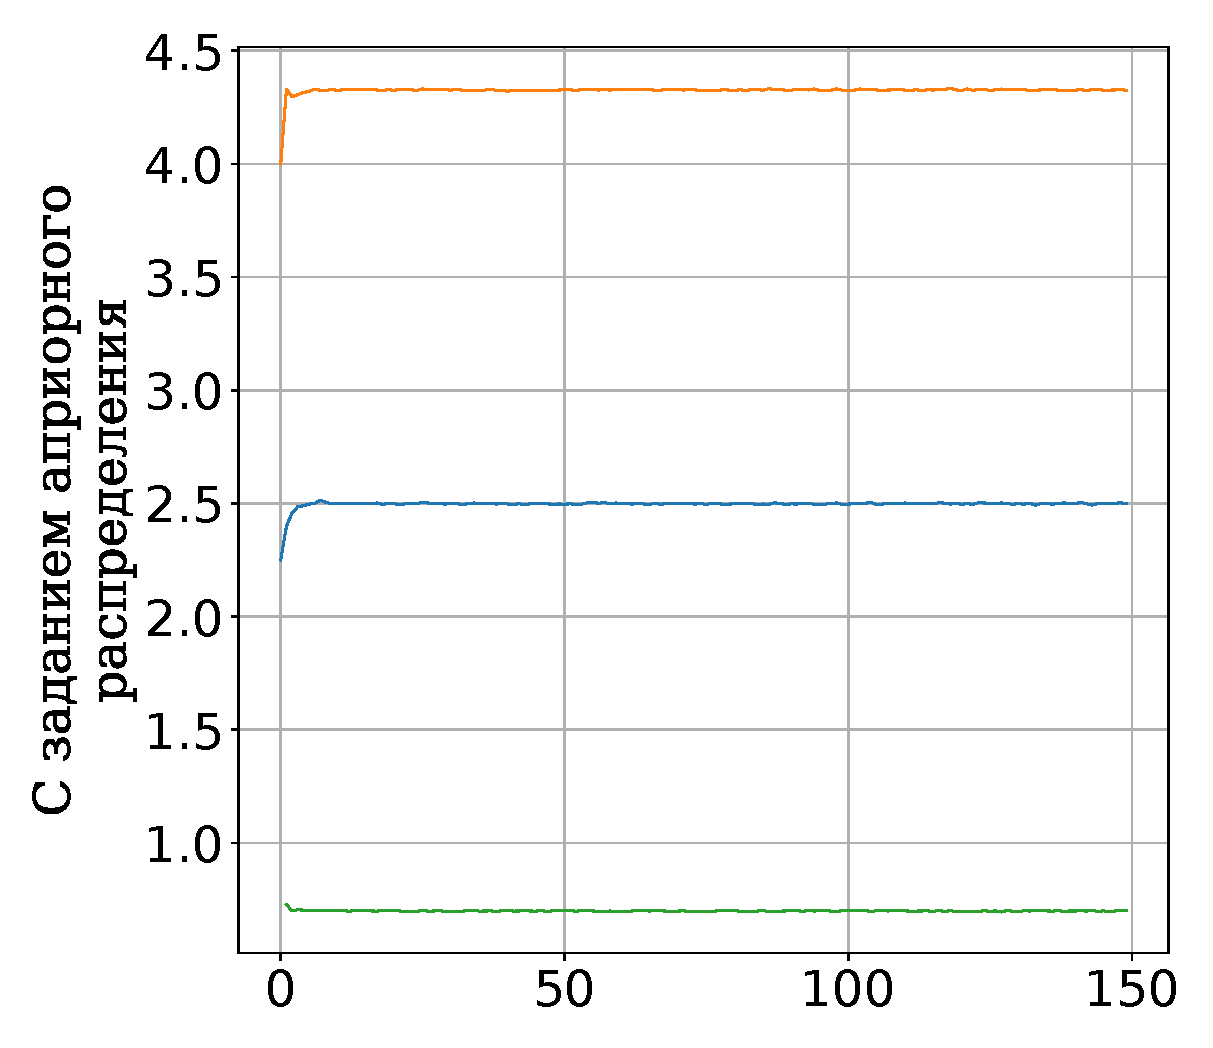
\includegraphics[width = 1.05\textwidth]{figures/910noise.eps}
\end{minipage}
\begin{minipage}{.32\textwidth}
\vspace{2pt}
\hspace{-2.1mm}
      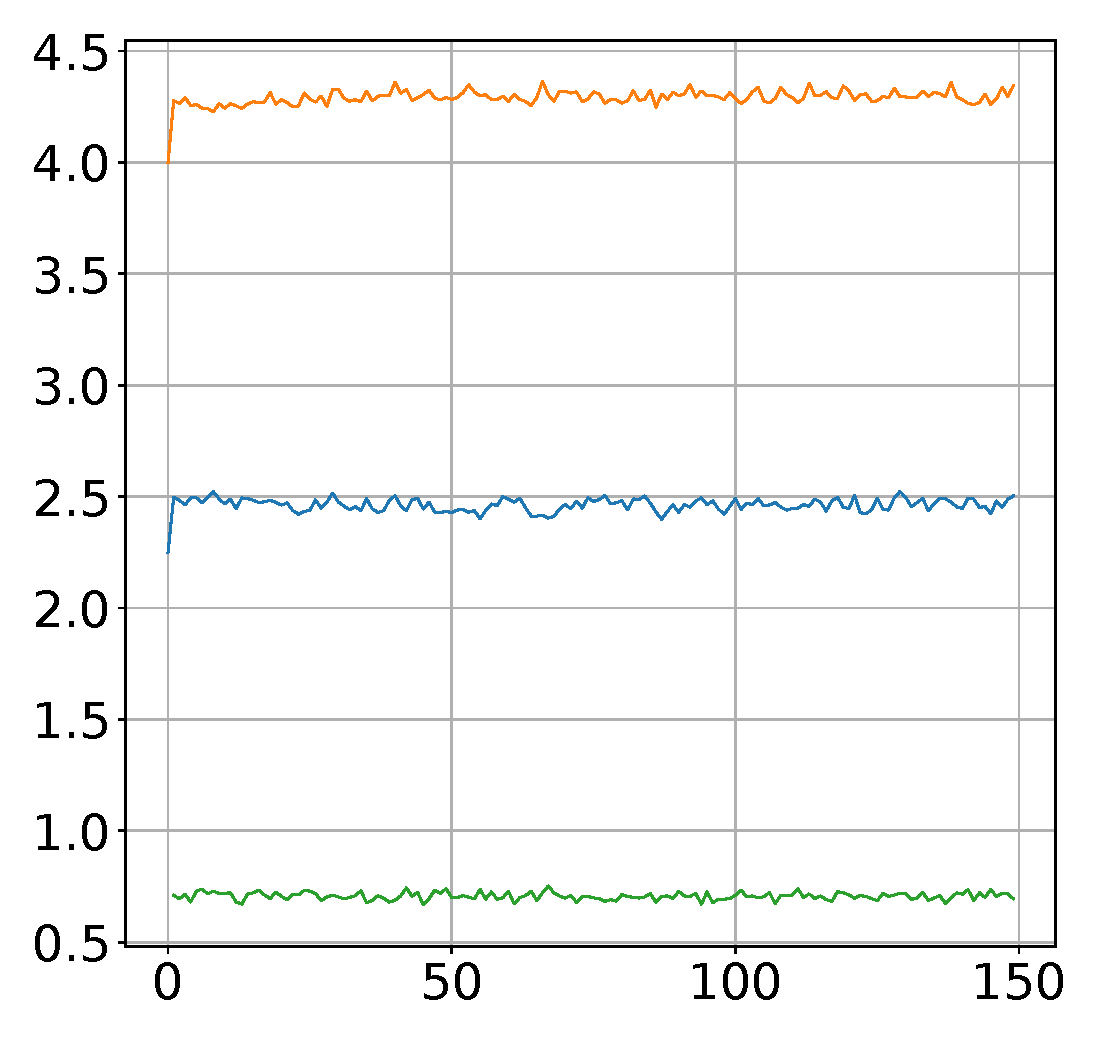
\includegraphics[width = 0.95\textwidth]{figures/911noise.eps}
\end{minipage}
\begin{minipage}{.32\textwidth}
\vspace{2pt}
\hspace{-6.3mm}
      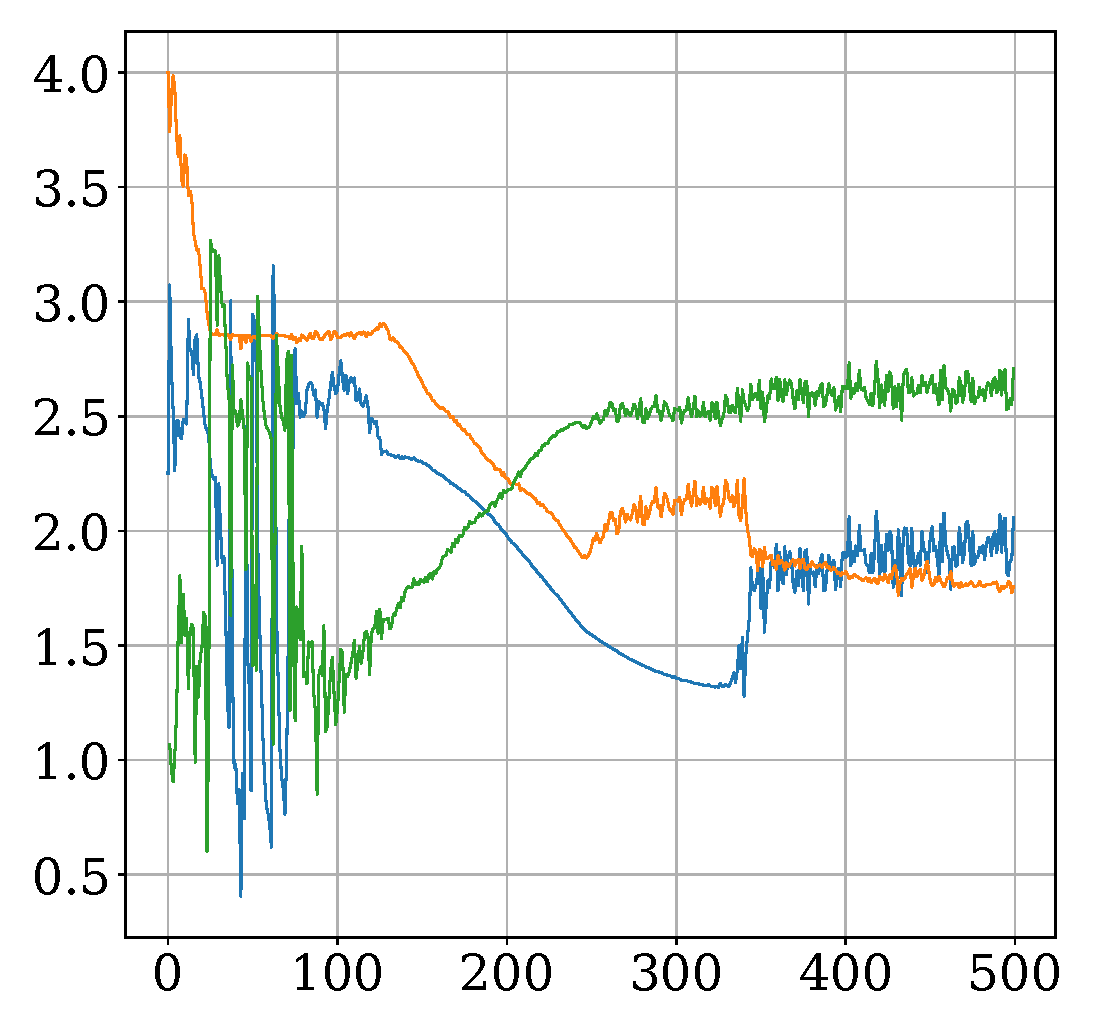
\includegraphics[width = 0.95\textwidth]{figures/912noise.eps}
\end{minipage}
\begin{minipage}{.32\textwidth}
\hspace{-3mm}
      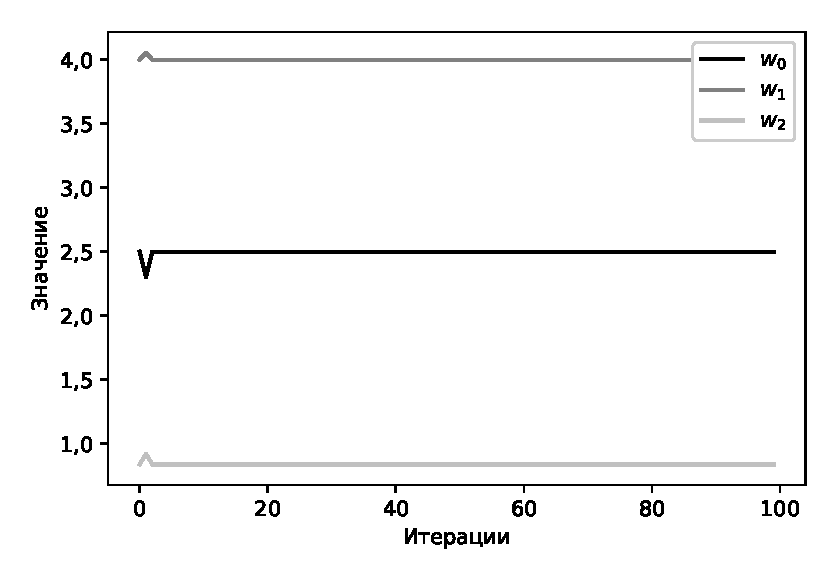
\includegraphics[width = 1.05\textwidth]{figures/900noise.eps}
\end{minipage}
\begin{minipage}{.32\textwidth}
\hspace{-2.1mm}
      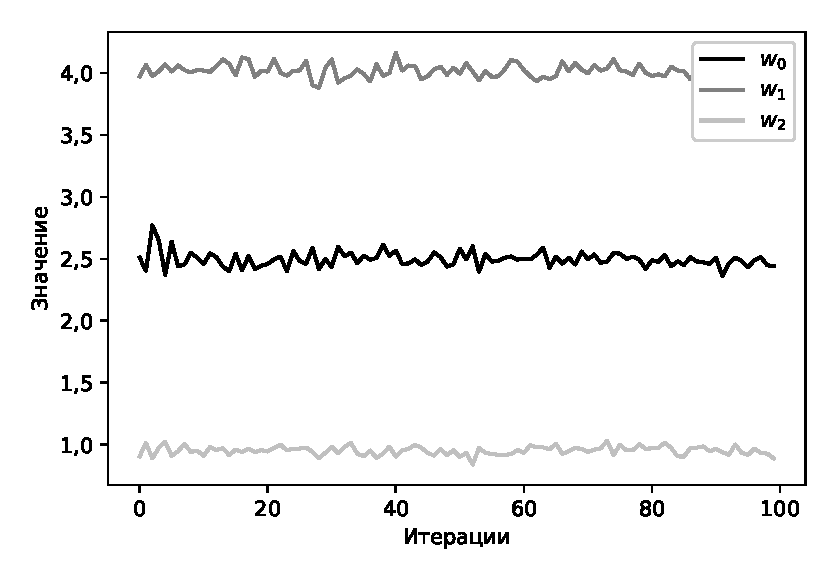
\includegraphics[width = \textwidth]{figures/901noise.eps}
\end{minipage}
\begin{minipage}{.32\textwidth}
\hspace{-2mm}
      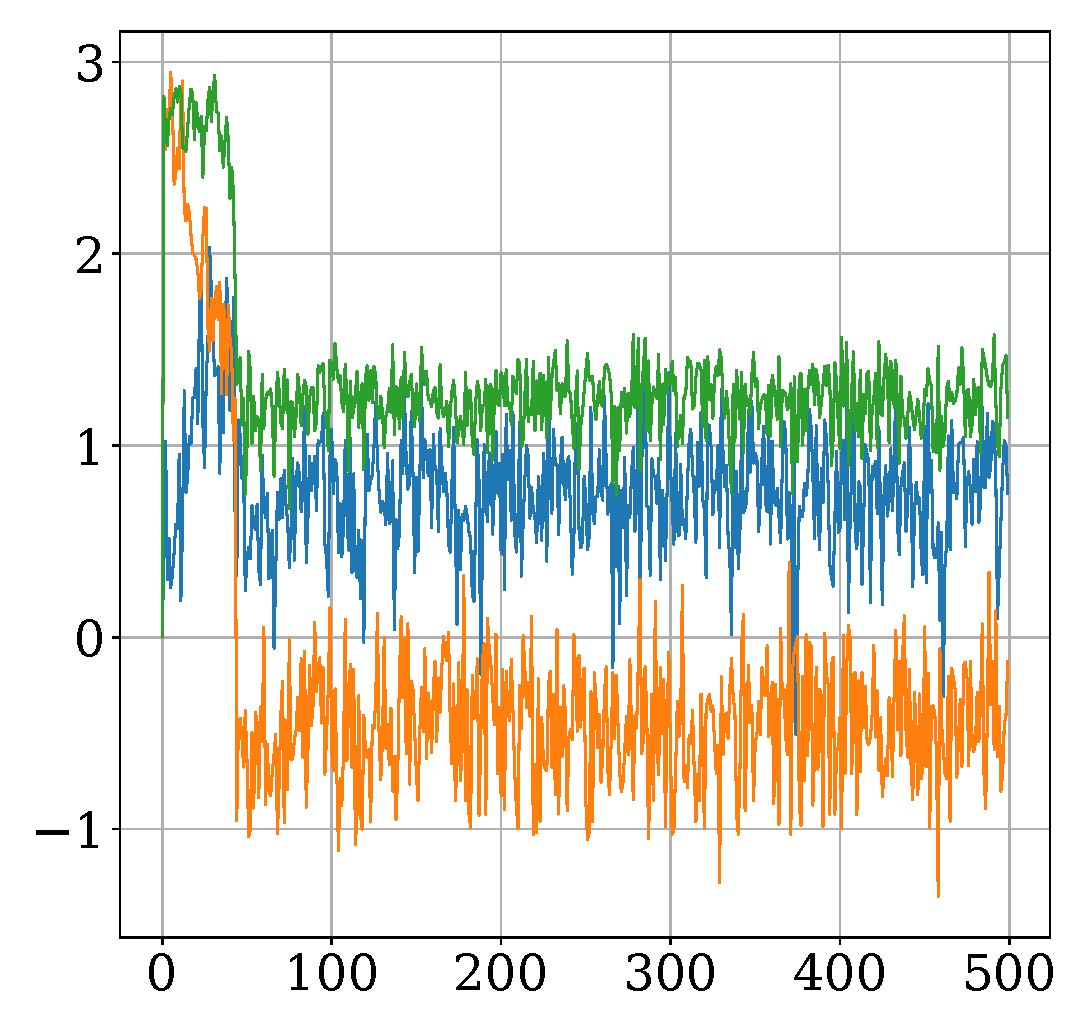
\includegraphics[width = 0.95\textwidth]{figures/902noise.eps}
\end{minipage}
\caption{Зависимость параметров $r$, $x_0$ и $y_0$ от номера итерации при разных априорных распределениях. Сверху вниз: построение с заданием априорного распределения; без задания априорного распределения. Слева на право: окружности без шума; шум в радиусе окружности; шум в радиусе окружности а также произвольные точки по всему изображению.}
\label{ce:fig4}
\end{figure}

В данной части эксперимента показан пример обучения мультимодели для аппроксимации нескольких фигур второго порядка одновременно. В качестве данных используется синтетическая выборка, которая получена при помощи генерации трех произвольных неперсекающихся окружностей, а также добавления к данным окружностям шума. Шум добавлялся к радиусу окружности для каждой точки, также в выборку были добавлены случайные точки, которые не относятся к окружностям. В эксперименте сравнивается две модели: в первой модели регуляризатор~$R\bigl(\mathbf{V}, \mathbf{W}, E(\Omega)\bigr)=0,$ то есть модель без задания регуляризатора, во второй модели регуляризатор:
\[
R\bigl(\mathbf{V}, \mathbf{W}, E(\Omega)\bigr)= -\sum_{k=1}^{K}\gamma\left(\mathbf{w}_k - \mathbf{w}_k^{0}\right)^{\mathsf{T}}\left(\mathbf{w}_k - \mathbf{w}_k^{0}\right),
\]
где~$\mathbf{w}_k^{0}$ априорные предположения о векторе параметров.

На рис.~\ref{ce:fig3} показан результат построения ансамбля локально аппроксимирующих моделей, которые аппроксимируют выборку. Каждая локальная модель аппроксимирует одну окружность, причем при добавления разного шума, качестве аппроксимации падет.
На рис.~\ref{ce:fig4} показан график зависимости радиуса окружностей $r$ и их центров $(x_0, y_0)$ от номера итерации. Видно, что модель с заданием априорного распределения сходится быстрее чем модель без задания априорного распределения.

\subsection{Эксперимент с разным уровнем шума и дисперсии априорного распределения}
\begin{figure}[h!t]\center
\includegraphics[width=0.8\textwidth]{figures/beta_gamma}
\caption{Результат аппроксимации для данных с разным уровнем шума~$\beta$ и от дисперсии априорного распределения~$\gamma$}
\label{ce:fig6}
\end{figure}

\begin{figure}[h!t]\center
\includegraphics[width=0.5\textwidth]{figures/3dplot}
\caption{Зависимость моделей от уровня шума~$\beta$ в данных, а также от дисперсии априорного распределения~$\gamma$}
\label{ce:fig5}
\end{figure}
В данной части эксперимента проводится анализ качества аппроксимации~$S$ от уровня шума~$\beta$ в данных и от параметра априорных распределений~$\gamma$. Выборка получена следующим образом: сначала случайным образом выбирается два вектора параметров~$\mathbf{w}^\text{true}_{1}$ и~$\mathbf{w}^\text{true}_{2}$ --- коэффициенты двух парабол. На основе векторов~$\mathbf{w}^\text{true}_{1}$ и~$\mathbf{w}^\text{true}_{2}$ выполняется генерация точек~$x_i$ и~$y_i$ с добавлением нормального шума~$\varepsilon\sim \mathcal{N}\bigr(0, \beta\bigr)$. При обучении мультимодели в качестве априорного распределения параметров рассматривается~$\mathbf{w}_1\sim\mathcal{N}\bigr(\mathbf{w}^\text{true}_{1}, \gamma\mathbf{I}\bigr),\mathbf{w}_2\sim\mathcal{N}\bigr(\mathbf{w}^\text{true}_{2}, \gamma\mathbf{I}\bigr)$.

Рассматривается следующий критерий качества:
\[
S = ||\mathbf{w}^\text{pred}_{1} - \mathbf{w}^\text{true}_{1}||^{2}_{2} + ||\mathbf{w}^\text{pred}_{2} - \mathbf{w}^\text{true}_{2}||^{2}_{2},
\]
где~$\mathbf{w}^\text{pred}_{1}$ аппроксимация вектора параметров первой локальной модели, а~$\mathbf{w}^\text{pred}_{2}$ аппроксимация вектора параметров второй локальной модели.

На рис.~\ref{ce:fig5} показана зависимость критерия качества~$S$ от уровня шума~$\beta$ и параметра априорного распределения~$\gamma$. Из графика видно, что при малом уровне шума~$\beta$ качество аппроксимации не зависит от параметра~$\gamma$, а при увеличении шума~$\beta$ качество аппроксимации~$S$ падает.

На рис.~\ref{ce:fig5} показан пример работы алгоритма при разных параметрах~$\beta$ и $\gamma$. Видно, что в случае отсутствия шума~$\beta$ обе локальные модели аппроксимируют выборку. При увеличении уровня шума качество аппроксимации падает: при~$\beta=0{,}2$ при увеличении $\gamma$ первая локальная модель из параболы переходит в эллипс; при~$\beta=0{,}4$ при увеличении  $\gamma$ первая локальная модель из параболы переходит в эллипс, а вторая модель из параболы переходит в гиперболу.

\subsection{Аппроксимации радужки глаза}
\begin{figure}
     \centering
     \begin{subfigure}[b]{0.3\textwidth}
         \centering
         \includegraphics[width=\textwidth]{figures/not_prior_real_example}
         \caption{}
     \end{subfigure}
     \begin{subfigure}[b]{0.3\textwidth}
         \centering
         \includegraphics[width=\textwidth]{figures/prior_real_example}
         \caption{}
     \end{subfigure}
     \begin{subfigure}[b]{0.3\textwidth}
         \centering
         \includegraphics[width=\textwidth]{figures/prior_regular_real_example}
         \caption{}
     \end{subfigure}
     \caption{Визуализация аппроксимации радужки глаза: a) в случае, если задан регуляризатор $R_0$; b) в случае, если задан регуляризатор $R_1$; b) в случае, если задан регуляризатор $R_2$.}
    \label{ce:fig6}
\end{figure}

\begin{figure}
     \centering
     \includegraphics[width=\textwidth]{figures/experiment_real_not_prior}\\
     
     \caption{Визуализация процесса сходимости мультимодели в случае регуляризатора~$R_0$}
    \label{ce:fig7}
\end{figure}

\begin{figure}
     \centering
     \includegraphics[width=\textwidth]{figures/experiment_real_prior}
     \caption{Визуализация процесса сходимости мультимодели в случае регуляризатора~$R_1$}
    \label{ce:fig8}
\end{figure}

\begin{figure}
     \centering
     \includegraphics[width=\textwidth]{figures/experiment_real_regular}
     \caption{Визуализация процесса сходимости мультимодели в случае регуляризатора~$R_2$}
    \label{ce:fig9}
\end{figure}

Проводиться анализ качества аппроксимации для задачи аппроксимации радужки глаза на изображении. Радужка глаза состоит из двух концентрических окружностей, поэтому рассматривается мультимодель, которая состоит из двух экспертов: каждый эксперт аппроксимирует одну из окружностей. В вычислительном эксперименте сравнивается качество аппроксимации окружностей в случае задания разных регуляризаторов $R_0, R_1, R_2$. Регуляризатор $R_0\bigl(\mathbf{V}, \mathbf{W}, E(\Omega)\bigr)=0,$ то есть регуляризатор отсутсвует. Регуляризатор:
\[
R_1\bigl(\mathbf{V}, \mathbf{W}, E(\Omega)\bigr)= -\sum_{k=1}^{K}\mathbf{w}_k^{\mathsf{T}}\mathbf{w}_k,
\]
который поощряет близкие к нулю параметры локальных моделей.
Регуляризатор
\[
R_2\bigl(\mathbf{V}, \mathbf{W}, E(\Omega)\bigr)= -\sum_{k=1}^{K}\mathbf{w}_k^{\mathsf{T}}\mathbf{w}_k + \sum_{k=1}^{K}\sum_{k'=1}^{K}\sum_{j=1}^2\left(w_k^j-w_k'^j\right)^2,\]
который поощряет совпадение центров окружностей и близкие к нулю параметры модели.
На рис.~\ref{ce:fig6} показан результат работы алгоритма аппроксимации радужки глаза после 10 итераций. Видно, что при отсутствии регуляризатора одна из окружностей находится не верно. В случае, если задан регуляризатор~$R_1$ модель аппроксимирует обе окружности с хорошим качеством, но окружности не являются концентрическими. В случае задания регуляризатор~$R_2$ получаем концентрические окружности на изображении.

На рис.~\ref{ce:fig7}-\ref{ce:fig9} показан процесс сходимости мультимоделей в случае задания разных регуляризаторов~$R_0,R_1,R_2$. Видно, что модели с типом регуляризатора~$R_1$ и~$R_2$ аппроксимируют обе окружности, а мультимодель с регуляризатором~$R_0$ аппроксимирует только большую окружность.


\section{Заключение}
В данной работе предложен метод для построения интерпретируемых моделей машиного обучения на основе экспертной информации. В качестве задачи рассмотрена задача аппроксимации кривых второго порядка: парабола, гипербола, эллипс. Аппроксимации кривых второго порядка применена в задачи аппроксимации радужки глаза.

Проведен эксперимент, в котором анализируется качество аппроксимации кривых второго порядка в зависимости от начального уровня шума в данных, а также в зависимости от регуляризатора. В ходе эксперимента показано, что при увеличении уровня шума в начальных данных, точность аппроксимации падает: при большом шума вид апроксимируемой фигуры изменяется с параболы на гиперболу.

Проведен вычислительный эксперимент по аппроксимации радужки глаза при помощи двух концентрических окружностей. В эксперименте показано, что регуляризация, которая основана на экспертной информации улучшает качество аппроксимации.

\begin{thebibliography}{99}
\bibitem{Ribeiro2016}
	\textit{Marco Tulio Ribeiro, Sameer Singh, Carlos Guestrin} "Why Should I Trust You?": Explaining the Predictions of Any Classifier // Proceedings of the 22nd ACM SIGKDD International Conference on Knowledge Discovery and Data Mining PP. 1135--1144. 2016

\bibitem{Tianqi2016}
	\textit{Chen Tianqi, Guestrin Carlos} XGBoost: A Scalable Tree Boosting System~// KDD ’16 Proceedings of the 22nd ACM SIGKDD International Conference on Knowledge Discovery and Data Mining. 2016.
	
\bibitem{Ishwaran2012}
	\textit{Chen Xi, Ishwaran Hemant} Random Forests for Genomic Data Analysis~// Genomics. 2012. Issues. 99, No 6. pp. 323--329.

\bibitem{Yuksel2012}
	\textit{Yuksel Seniha Esen, Wilson Joseph N., Gader Paul D} Twenty Years of Mixture of Experts~// IEEE Transactions on Neural Networks and Learning Systems. 2012. Issues. 23, No 8. pp. 1177--1193.


\bibitem{Cao2003}
	\textit{L.~Cao} Support vector machines experts for time series forecasting~// Neurocomputing, vol. 51, pp. 321–339, Apr. 2003.

\bibitem{Dempster1977}
	\textit{A. P. Dempster, N. M. Laird and D. B. Rubin} Maximum Likelihood from Incomplete Data via the EM Algorithm~// Journal of the Royal Statistical Society. Series B (Methodological), Vol. 39, No. 1 pp. 1-38, 1977.
	
	
\bibitem{Yumlu2003}
	\textit{M.\,S.~Yumlu, F.\,S.~Gurgen,  N.~Okay} Financial time series prediction using mixture of experts~// in Proc. 18th Int. Symp. Comput. Inf. Sci., 2003, pp. 553--560.
	
\bibitem{Cheung1995}
	\textit{Y.~M.~Cheung, W.~M.~Leung, and L. Xu} Application of mixture of experts model to financial time series forecasting~// in Proc. Int. Conf. Neural Netw. Signal Process., 1995, pp. 1--4.
	
\bibitem{Weigend2000}
	\textit{A. S. Weigend, S. Shi} Predicting daily probability distributions of S\&P500 returns~// J. Forecast., vol. 19, no. 4, pp. 375--392, 2000.
	
\bibitem{Ebrahimpour2009}
	\textit{R. Ebrahimpour, M. R. Moradian, A. Esmkhani, F. M. Jafarlou} Recognition of Persian handwritten digits using characterization loci and mixture of experts~// J. Digital Content Technol. Appl., vol. 3, no. 3, pp. 42–46, 2009.
	
\bibitem{Estabrooks2001}
	\textit{A.~Estabrooks, N.~Japkowicz} A mixture-of-experts framework for text classification~//in Proc. Workshop Comput. Natural Lang. Learn., Assoc. Comput. Linguist., 2001, pp. 1--8.
	
\bibitem{Mossavat2010}
	\textit{S. Mossavat, O. Amft, B. de Vries, P. Petkov, W. Kleijn} A Bayesian hierarchical mixture of experts approach to estimate speech quality~// in Proc. 2nd Int. Workshop Qual. Multimedia Exper., pp. 200--205., 2010
	
\bibitem{Sminchisescu2007}
	\textit{C. Sminchisescu, A. Kanaujia, and D. Metaxas} B M3 E: Discrimina- tive density propagation for visual tracking~// IEEE Trans. Pattern Anal. Mach. Intell., vol. 29, no. 11, pp. 2030–2044, 2007.
	
\bibitem{Matveev2010}
	\textit{I. Matveev} Detection of iris in image by interrelated maxima of brightness gradient projections~// Appl.Comput. Math. 9 (2), 252–257, 2010.

\bibitem{Matveev2014}
	\textit{I. Matveev, I. Simonenko}. Detecting precise iris boundaries by circular shortest path method~// Pattern Recognition and Image Analysis. 24. 304-309. 2014.
	
\bibitem{Bowyer2010}
	\textit{K. Bowyer, K. Hollingsworth, P. Flynn} A Survey of Iris Biometrics Research: 2008–2010.

\bibitem{Peng1996}
	\textit{F. Peng, R. A. Jacobs, M. A. Tanner} Bayesian inference in mixtures-of-experts and hierarchical mixtures-of-experts models with an application to speech recognition~// J. Amer. Stat. Assoc., vol. 91, no. 435, pp. 953–960, 1996.
	
\bibitem{Tuerk2001}
	\textit{A. Tuerk} The state based mixture of experts HMM with applications to the recognition of spontaneous speech~// Ph.D. thesis, Dept. Eng., Univ. Cambridge, Cambridge, U.K., 2001.
	
\bibitem{bishop2006}
	\textit{Bishop C.} Pattern Recognition and Machine Learning.~---~Berlin: Springer, 2006. 758~p.

\bibitem{Kaiming2015}
	\textit{Kaiming He} Deep Residual Learning for Image Recognition.
	
\bibitem{Han2020}
	\textit{Han Xu} Adversarial Attacks and Defenses in Images, Graphs and Text: A Review
	
\bibitem{Xingjun2019}
	\textit{Xingjun Ma} Understanding Adversarial Attacks on Deep Learning Based Medical Image Analysis Systems
	
\bibitem{Akhtar2018}
	\textit{Naveed Akhtar} Threat of Adversarial Attacks on Deep Learning in Computer Vision: A Survey
	
\bibitem{Dalila2018}
	\textit{Salamani Dalila} Deep generative models for fast shower simulation in ATLAS
	
 \end{thebibliography}


\end{document}

